\qns{Nonlinear Pendulum}

In this question, we'll take a look at a nonlinear system that cannot be written in state-space, and linearize it around an equilibrium point to create a linear approximation.

Consider the damped pendulum shown below, where the pendulum has length $L$ and makes an angle $\theta$ with the vertical axis:
\begin{center}
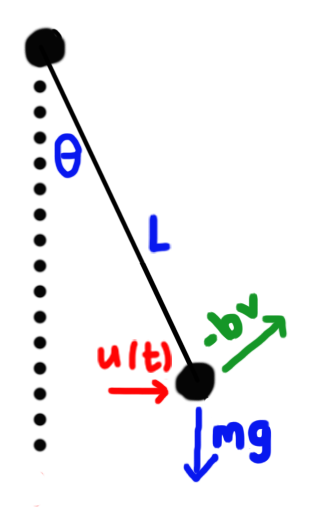
\includegraphics[scale=0.3]{\bank/linearization/figures/pendulum.png}
\end{center}
The kinetics of this pendulum over time can be represented by the following differential equation:
\begin{equation}
  \frac{d^{2} \theta}{dt^{2}} = -\frac{g}{L} \sin \theta - \frac{b}{m} \ddt{\theta}{t} + \frac{\cos \theta}{mL} u
\end{equation}
Where $m$ is the mass of the pendulum, $g$ is gravitational acceleration, $b$ is a damping coefficient due to air resistance, and $u(t)$ is an input force on the pendulum. We will also define the following state-variable $\vec{x}$ 
\begin{equation*}
  \vec{x} = \begin{bmatrix} x_{1} \\ x_{2} \end{bmatrix} = \begin{bmatrix} \theta \\ \omega \end{bmatrix} = \begin{bmatrix} \theta \\ \ddt{\theta}{t} \end{bmatrix}
\end{equation*}

If we try putting this system into state-space form we will see that it is impossible since the system is nonlinear.
Therefore, we will use our knowledge of linearization to linearize this system.

Recall that a nonlinear system $\ddt{}{t} \vec{x}(t) = f(\vec{x}, u)$ can be linearized as:
\begin{equation}
  \ddt{}{t} \vec{\delta}_{\vec{x}}(t) = J_{\vec{x}} \ \vec{\delta}_{\vec{x}}(t) + J_{u} \ \delta_{u}(t)
\end{equation}
where $J_{\vec{x}}$ and $J_{u}$ are the respective Jacobians of $f$ with respect to $\vec{x}$ and $u.$

\begin{enumerate}
  \qitem How can you write $\ddt{}{t} \vec{x}(t) = f(\vec{x}, u)$ as a vector differential equation?

  \sol {
    $$\ddt{}{t} \vec{x} 
    = \ddt{}{t} \begin{bmatrix} \theta \\ \ddt{\theta}{t} \end{bmatrix} 
    = \ddt{}{t} \begin{bmatrix} f_{1}(\vec{x}, u) \\ f_{2}(\vec{x}, u) \end{bmatrix}
    = \begin{bmatrix} \ddt{\theta}{t} \\ -\frac{g}{L} \sin \theta - \frac{b}{m} \ddt{\theta}{t} \end{bmatrix} + 
      \begin{bmatrix} 0 \\ \frac{\cos \theta}{m \cdot L} \end{bmatrix} u(t)$$
  }

  \qitem What are $J_{\vec{x}}$ and $J_{u}$ evaluated the equilibrium points $\vec{x}^{*} = \begin{bmatrix} 0 \\ 0 \end{bmatrix}, u^{*} = 0.$

  \meta {
    You may want to discuss the shape of the Jacobians, and why the Jacobian for $\vec{x}$ is a $2 \times 2$ matrix while the Jacobian for $u$ is a $2 \times 1$ vector.
  }

  \sol {
    The indivdual functions $f_{1}, f_{2},$ in terms of the state variables $x_1, x_2$ and the input $u$ are
    \begin{align*} 
      &f_{1}(x_{1}, x_{2}, u) = x_{2} \\
      &f_{2}(x_{1}, x_{2}, u) = -\frac{g}{L} \sin x_{1} - \frac{b}{m} x_{2} + \frac{\cos{\theta}}{mL} u
    \end{align*}

    The Jacobian for $\vec{x}$ is:
    $$J_{\vec{x}} =
    \begin{bmatrix} \frac{\partial f_{1}}{\partial x_{1}} & \frac{\partial f_{1}}{\partial x_{2}} \\
    \frac{\partial f_{2}}{\partial x_{1}} & \frac{\partial f_{2}}{\partial x_{2}}
    \end{bmatrix} = 
    \begin{bmatrix} 0 & 1 \\
    -\frac{g}{L} \cos x_{1} & -\frac{b}{m} 
    \end{bmatrix} = 
    \begin{bmatrix} 0 & 1 \\
    -\frac{g}{L} \cos \theta & -\frac{b}{m} 
    \end{bmatrix}
    $$
    The Jacobian for $u$ is:
    $$J_{u} =
    \begin{bmatrix} \frac{\partial f_{1}}{\partial u} \\ \frac{\partial f_{2}}{\partial u} \end{bmatrix} =
    \begin{bmatrix} 0 \\ \frac{\cos x_{1}}{mL} \end{bmatrix} = 
    \begin{bmatrix} 0 \\ \frac{\cos \theta}{mL} \end{bmatrix}
    $$
    Evaluating at the operating point, $\vec{x}^{*}, u^{*}$ we get:
    $$J_{\vec{x}} |_{\vec{x} = \vec{x}^{*}} =
    \begin{bmatrix} 0 & 1 \\
    -\frac{g}{L} & -\frac{b}{m} 
    \end{bmatrix} \hspace{0.3 cm}
    J_{u} |_{u = u^{*}} =
    \begin{bmatrix} 0 \\ \frac{1}{mL} \end{bmatrix}
    $$
  }

  \qitem Using these Jacobians, construct the new linearized system in state-space form.

  \sol {
    The state-space form will be:
    $$\ddt{}{t} \delta_{x}(t) = 
    \begin{bmatrix} 0 & 1 \\
    -\frac{g}{L} & -\frac{b}{m} 
    \end{bmatrix} \vec{\delta}_{\vec{x}}(t) + 
    \begin{bmatrix} 0 \\ \frac{1}{mL} \end{bmatrix} \vec{\delta}_{u}(t)
    $$
  }

  \qitem What are the eigenvalues of this system?

  \sol {
    The eigenvalues of this system, are the eigenvalues of the $J_{\vec{x}}$ matrix:
    $$\begin{bmatrix} 0 & 1 \\
    -\frac{g}{L} & -\frac{b}{m} 
    \end{bmatrix}$$
    The determinant of $J_{\vec{x}} - \lambda I$ is:
    $$\text{det} \bigg( \begin{bmatrix} -\lambda & 1 \\
    -\frac{g}{L} & -\frac{b}{m} -\lambda
    \end{bmatrix} \bigg) = (-\lambda)(-\frac{b}{m} - \lambda) + \frac{g}{L} = \lambda^{2} + \frac{b}{m} \lambda + \frac{g}{L}$$
    The eigenvalues are the roots of this characteristic polynomial:
    $$\lambda = -\frac{b}{2m} \pm \frac{1}{2} \sqrt{\big( \frac{b}{m} \big)^{2} - \frac{4g}{L}}$$
  }

  \qitem Under what conditions is this system stable? Is is stable when $b = 2, \ m = 2, \ g = 10, \ L = \frac{1}{2}?$

  \meta {
    Note that $g$ and $L$ do not affect stability, and will only affect the damping of the system.
    They may cause the eigenvalues to be complex, but the imaginary part of eigenvalues do not affect stability.
  }

  \sol {
    Remember that a system is stable, when $\mathfrak{Re}(\lambda_{i}) < 0$ for all $i.$
    For this system, $\mathfrak{Re}(\lambda_{1}) = \mathfrak{Re}(\lambda_{2}) = -\frac{b}{2m}$ meaning the system will be stable when $\frac{b}{2m} > 0.$
    Therefore, the system is indeed stable, when $b = 2$ and $m = 2.$ 
  }

  \qitem Is this system controllable?

  \meta {
    You are allowed to claim this system is controllable since it is in Controllable Canonical Form, but we'll do the derivation through the controllability matrix $\mathcal{C}$ anyway.
  }

  \sol {
    We can claim that this system is controllable, since it is in Controllable Canonical Form. 
    Alternatively we can also compute the controllability matrix as:
    $$\mathcal{C} = 
    \begin{bmatrix} 
    0 & \frac{1}{mL} \\
    \frac{1}{mL} & -\frac{b}{m^{2} L}
    \end{bmatrix}$$
    Since $\frac{1}{mL}$ cannot be zero, the second column cannot be a scalar multiple of the first. 
    Therefore, the controllability matrix is full rank, and the system is controllable.
  }

  \qitem Now suppose that there is a strong wind pushing our pendulum which changes the dynamics so that $b = -2.$ 
  Show that this system is unstable.

  \meta {
    Remember that linearization is an approximation to a system at a given operating point.
    Since the linearization is defined in terms of $\delta_{\vec{x}}(t),$ the distance from the operating point, 
    if a linearization is unstable, it means that the error of the approximation will be unbounded as you get farther away from the operating point.
  }

  \sol {
    Since $b = -2, \mathfrak{Re}(\lambda_{1}) = \mathfrak{Re}(\lambda_{2}) = \frac{1}{2} \geq 0$ which implies the system is unstable.
  }

  \qitem Show that the system is in Controllable Canonical Form for the given physical values: $b = -2, \ m = 2, \ g = 10, \ L = \frac{1}{2}.$

  \sol {
    Plugging these values in, we see that the system is indeed in Controllable Canonical Form:
    $$\ddt{}{t} \delta_{x}(t) = 
    \begin{bmatrix} 
    0 & 1 \\
    -20 & 1
    \end{bmatrix} \vec{\delta}_{\vec{x}}(t) + 
    \begin{bmatrix} 0 \\ 1 \end{bmatrix} \vec{\delta}_{u}(t)
    $$
  }

  \qitem  We will use the fact that this system is in Controllable Canonical Form to stabilize the system. 
  Design a feedback controller so that the eigenvalues of the system will be $\lambda_{1} = -2, \ \lambda_{2} = -3.$

  \sol {
    Setting $u = K \vec{\delta}_{\vec{x}}(t)$ as the input, where $K = \begin{bmatrix} k_{1} & k_{2} \end{bmatrix},$
    the closed-loop matrix will be:
    $$A_{cl} = \begin{bmatrix}
    0 & 1 \\
    -20 + k_{1} & 1 + k_{2}
    \end{bmatrix}$$
    We know that the characteristic polynomial of this matrix will be $\lambda^{2} - (1 + k_{2}) \lambda - (-20 + k_{1}).$
    To make the eigenvalues $-2$ and $-3,$ we want our characteristic polynomial to be $\lambda^{2} + 5 \lambda + 6$ so picking $k_{1} = 14$ and $k_{2} = -6$ will suffice.
  }

\end{enumerate}